\documentclass[%
%   preprint,
superscriptaddress,
%groupedaddress,
%unsortedaddress,
%runinaddress,
%frontmatterverbose,
%preprint,
%showpacs,preprintnumbers,
%nofootinbib,
%nobibnotes,
%bibnotes,
%twocolumn,
amsmath,amssymb,
aps,
pre,
%prb,
%rmp,
%prstab,
%prstper,
floatfix,
]{revtex4-2}

\usepackage{graphicx}% Include figure files
\usepackage{dcolumn}% Align table columns on decimal point
\usepackage{bm}% bold math
\usepackage{hyperref}% add hypertext capabilities
\usepackage{color}
\usepackage{verbatim}
\graphicspath{{./fig/}}
%\usepackage{epstopdf}
%\usepackage{auto-pst-pdf}


\begin{document}
\title{Toy model for the sawtooth oscillation}
\author{Ralf Mackenbach}
\affiliation{Princeton Plasma Physics Laboratory, Princeton University, Princeton, New Jersey, USA}
\author{C. B. Smiet}
\affiliation{Princeton Plasma Physics Laboratory, Princeton University, Princeton, New Jersey, USA}
\affiliation{Huygens-Kamerlingh Onnes Laboratory, Leiden University, P.O.\ Box 9504, 2300 RA Leiden, The Netherlands}

\begin{abstract}
  The Sawtooth crash is an instability occurring in the core of a tokamak plasma that redistributes the temperature and pressure in the core region.
  In the Kadomtsev model the crash is caused by a 1/1 internal kink that reconnects the hot plasma within the core region.
  In this paper we present a minimal analytical model with two free parameters that reproduces the predicted changes in topology.
  This paints an intuitive picture of how the magnetic topology changes during a sawtooth crash.
\end{abstract}
\maketitle

The sawtooth crash has been observed in tokamak fusion reactors since 1974 \cite{von1974studies, vershkov1974role}.
Because of the temperature dependent Spitzer resistivity, the plasma current that creates the rotational transform in the reactor preferentially concentrates on the hottest plasma region near the magnetic axis.
This decreases the safety factor (increases the field line winding) around the core.
Current diffuses onto the core of the tokamak on a slow, resistive timescale, until a fast instability is triggered at a specific value of $q_0$ (the safety factor on the magnetic axis)
At a specific value of $q_0$ a fast instability is triggered that redistributes the plasma in the core region, and leads to a flat temperature and pressure profile.
This instability redistributes the poloidal and toroidal flux, resulting in a higher $q_0$.
The sawtooth cycle resets, and current slowly accumulates on the axis until the instability is triggered again.

One of the most enduring models for the sawtooth was presented by Kadomtsev~\cite{kadomtsev1975disruptive}.
In this model the region within the $q=1$ surface becomes susceptible to an internal kink mode, a resistive tearing instability of the $q=1$ surface, or both~\cite{coppi1976resistive}.
The plasma in the core reconnects with cold plasma from outside the $q=1$ surface along a helical ribbon on the $q=1$ surface, and is deposited in a growing 1/1 island.
This growing island eventually completely displaces the hot core, and the temperature and current are re-distributed.
After the crash, the hot core is completely replaced by the $1/1$ island, which has $q_0=1$.

In this paper we present a simple analytical toy model for the above process that uses two independent parameters to reproduce the predicted change in topology: a 1/1 internal kink that displaces the core, and a linear interpolation between the initial and final flux predicted by kadomtsev.
Other expressions for the time-dependent magnetic topology during the sawtooth crash have been presented by Kolesnichenko~\cite{kolesnichenko1996theory} and Jaulmes~\cite{jaulmes2014redistribution}.
These works calculate the intermediate states in the Kadomtsev reconnection process, whereas the current treatment separates the reconnection phase into two separate and independent perturbations, resulting in a more analytically tractable and intuitive picture, at the cost of accuracy.

\section*{Fields}
The magnetic field in a tokamak ideally consists of nested toroidal magnetic surfaces with a monotonically increasing $q$-profile.
We generate such an equilibrium field using a poloidal flux function $\psi_p(R, Z)$ and a toroidal current function $I(\psi_p)$.
The coordinates used are illustrated in figure~\ref{fig:coords}.
Physically $\psi_p$ represents the amount of flux through the circular disc with radius R centered on the $Z$ axis (indicated by the green circle in figure~\ref{fig:coords}.
$I$, which is sometimes called $F$ or $G$, represents the current through the same surface divided by 2$\pi$.
\begin{figure}\label{fig:coords}
  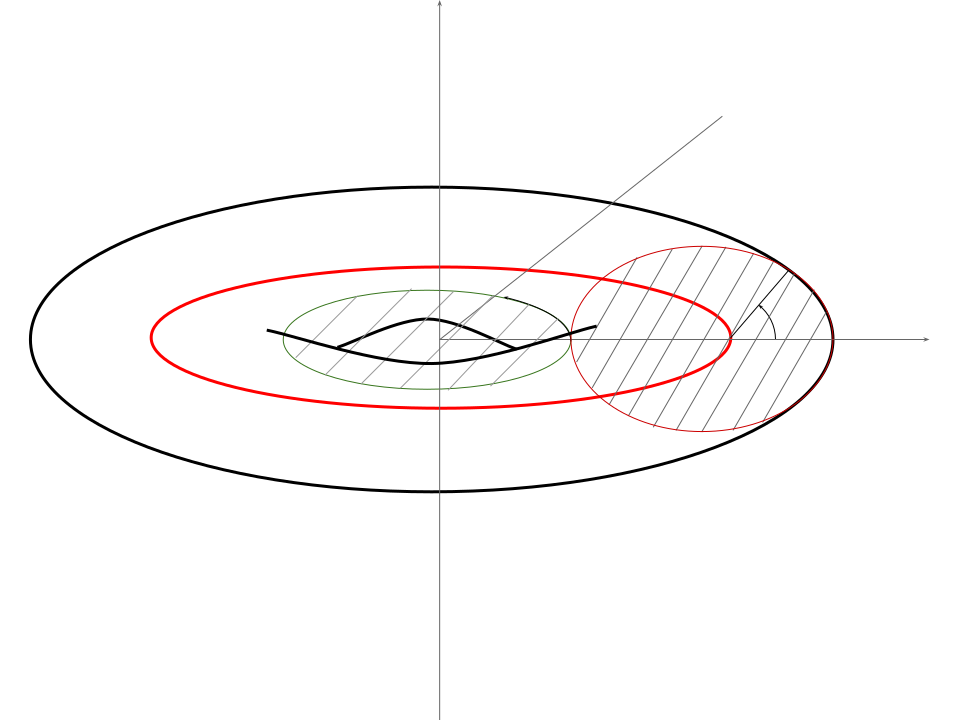
\includegraphics[0.5\textwidth]{fig/torus.svg}
  \caption{Coordinates used for generating the magnetic field. }
\end{figure}

The magnetic fields are calculated from $\psi_p$ and $I$ using:
\begin{equation}
  B_R = -\frac{1}{R} \frac{\partial \psi_p}{\partial z}, \quad B_z= \frac{1}{R} \frac{\partial
  \psi_p}{\partial R}, \quad
  B_\phi = \frac{1}{R} I.
\end{equation}

For the poloidal flux function we use
\begin{equation}
  \psi_p = a^2
\end{equation}
where $a=\sqrt{Z^2 + (R-R_0^2}$ with $R_0$ the location of the magnetic axis.
The surfaces of constant $\psi_p$, which are magnetic surfaces, are thus circular-cross-section concentric tori around a magnetic axis located at $R=R_0$.

For our current function $I$ we choose the following relation:
\begin{equation}
  I(\psi) = 2(q_0 + \alpha \psi_p)\sqrt{R_0-psi_p}
\end{equation}


The safety factor on each surface is calculated through~\cite{wesson2011tokamaks}:
\begin{equation}\label{eq:qprofint}
  q=\frac{1}{2\pi} \oint \frac{1}{R}\frac{B_\theta}{B_p}\dd l,
\end{equation}
where $B_p=\sqrt(B_R^2+B_Z^2}$ is the poloidal magnetic field.
The integration is carried out over a magnetic surface, which in the circular-cross-section concentric toroidal geometry can be done analytically.
The quantity $R B_p$ is constant in this geometry, so we get:
\begin{equation}
  q = \frac{1}{2\pi} \frac{I(psi_p)}{RB_p}\oint \frac{1}{R} \mathrm{d}l.
\end{equation}
We evaluate the integral by integrating over $\theta$ and using the identities $R=R_0 +a \cos(\theta)$ and $\mathrm{d}l = a \mathrm{d}\theta$ to yield:
\begin{equation}
  \oint \frac{1}{R} \mathrm{d}l = /int_0^{2\pi} \frac{a}{R_0 + a \cos(\theta)} \mathrm{d}l =
  \frac{2\pi a}{sqrt{R_0^2 -a^2}}
\end{equation}
In the above integration we used the facts that $R_0>0$ and $R_0>a>0$.
This explains our choice of the function $I$, whose square root term cancels against the integrand, giving us the safety factor profile of:
\begin{equation}
  q=q_0 + \alpha \psi_p.
\end{equation}.

The expressions derived above thus give us an axisymmetric magnetic field where field lines lie on nested concentric toroidal magnetic surfaces.
This field has no shafranov shift (a shift of the magnetic axis outwards, induced by plasma pressure).
Including a shafranov shift would make the factor $RB_p$ non-constant on a magnetic surface, thus requiring numerical integration for the evaluation of the integral in~\ref{eq:qprofint}.





\bibliographystyle{naturemag}
\bibliography{refs}

\end{document}
